% ----------------------------------------
% Chap: Konstruktive Bearbeitung
% ----------------------------------------
\chapter{Konstruktive Bearbeitung}
\label{chap:konstruktive_bearbeitung}

Um die Messgenauigkeit der optischen Interferometrie-Technik mit der einfachen Adaptierbarkeit an verschiedenen realen Maschinenelementen der elektrischen Messmethode zur Schmierfilmdickenmessung im EHD-Kontakt zu vereinigen, soll ein neues modular Messsystem auf Basis des EHD-Prüfstands von PCS entwickelt werden.
Dies System soll die optische und elektrische (kapazitive) Messung gleichzeitig erlauben.
Für solches System gibt es die folgende Anforderungen, die durch konstruktive Bearbeitung in nächsten Abschnitten gelöst werden.
\begin{itemize}
    \item Elektrische Isolierung der Glasscheibe und der Kugel mit dem gesamten System.
    \item Elektrische Zugänge für die Messproben an der Scheibe und der Kugel.
    \item Beschichtung auf der Scheibe, die elektrische und optische Messung gleichzeitig erlaubt.
\end{itemize}

% ----------------------------------------
% Sec: Konstruktion der Kugelführung
% ----------------------------------------
\section{Konstruktion der Kugelführung}
\label{sec:konstruktion_der_kugelfuehrung}

Da das modifizierte Kugelsupport mit einstellbarer Achse von \textit{E. Wittek} \cite{wittek_2007} wegen Rundlaufabweichung nur bis Wälzgeschwindigkeit von c.a 0,7 $m/s$ einsetzbar ist, wird das Prinzip der originalen Kugelführung der PCS Firma im Rahmen dieser Arbeit weiter benutzt.
Bei der standardmäßigen Kugelführung wird eine durchgebohrte Kugel in einem Adapter eingeklemmt, welche dann über einen Querstift mit der Motorausgangswelle des zweiten Antriebs formschlüssig verbunden wird.
Für die kapazitive Messung soll die Kugel elektrisch mit dem gesamten System isoliert werden, das erfolgt durch die Verwendung eine Kunststoffwelle.
Die Kugelaufnahme wird aus Messing gefertigt, um den Kontaktwiderstand mit den zu Signal übertragenden Kohlebürsten zu reduzieren.
Die Abbildung \ref{fig:aufbau_der_neuen_kugelfuehrung} zeigt den Zusammenbau der neuen Kugelführung.
% ----------------------------------------
% Fig: Aufbau der neuen Kugelführung
% ----------------------------------------
\begin{figure}[htb]
    \centering
    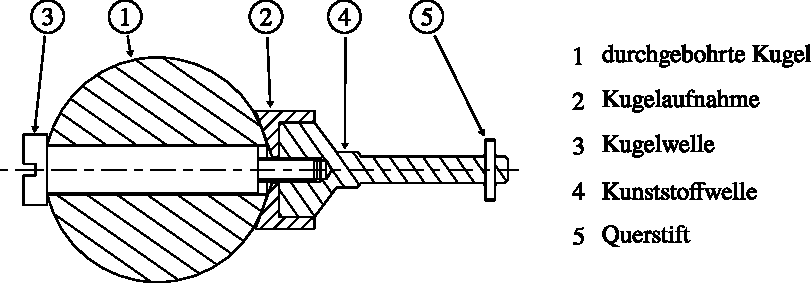
\includegraphics[]{./images/durchgebohrte_kugel.pdf}
    \caption{Aufbau der neuen Kugelführung}
    \label{fig:aufbau_der_neuen_kugelfuehrung}
\end{figure}
%

Die geführte Kugelachse ermöglicht die Versuche mit Schlupf und verhindert auch das unkontrollierte Einbringen des Schmierstoffes (Öl, Fett) in den Kontakt.
Der Kraftfluss zwischen dem zweiten Motor und der Kugel kann durch den Wegfall des Querstifts unterbrochen werden.
In diesem Fall dreht sich die Kugelführung frei in der Motorausgangswelle.

% ----------------------------------------
% Sec: Konstruktion des Kugelsupports
% ----------------------------------------
\section{Konstruktion des Kugelsupports}
\label{sec:konstruktion_des_kugelsupports}

Das originale Kugelsupport von PCS ist relativ kompakt und simpel konstruiert, aus diesem Grund wird es für die elektrische Messung modifiziert und weiter benutzt.

Das neue Kugelsupport (Abbildung \ref{fig:das_modifizierte_kugelsupport}) besteht aus drei Rillenkugellager, die auf einem dreieckigen Klotz befestigt werden.
Die Kugel wird von den drei Lagern sicher von unten gegen der Glasscheibe gestützt.
Da die Kugel mit der Lasteinheit elektrisch isoliert werden muss, ist der Klotz aus Kunststoff gefertigt.
Auf der Unterseite des Klotzs befinden sich zwei Löcher, die mit den Stifte der Lasteinheit arretiert werden, dadurch wird die Position des Kugelsupports während Versuche sicher gestellt.
An der Seite des Supports sind zwei M3 Bohrung zur Anbringung der Kohlebürstenhalter, die für die Aufnahme der elektrischen Signale von der Kugel zuständig sind, zu versehen.
Bei der Versuchen mit Fett ist dort auch möglich, die Befettungsvorrichtung zu montieren.
% ----------------------------------------
% Fig: Das modifizierte Kugelsupport
% ----------------------------------------
\begin{figure}[htb]
    \centering
    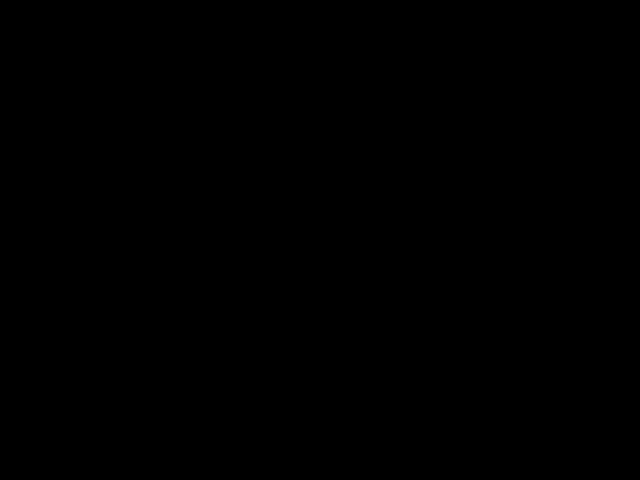
\includegraphics[width=4cm]{./images/blank_img.jpg}
    \caption{Das modifizierte Kugelsupport}
    \label{fig:das_modifizierte_kugelsupport}
\end{figure}
%

Der Kohlebürstenhalter ist aus Messing, hat eine zylindrische Form und wird mit einem Blechhalter, welcher an der Seite des Supports angeschraubt wird, gelötet.
Die Kohlebürste Typ \textit{KK399} wurden von der Firma \textit{Schmidthammer} gekauft.
Dank dem hohen Kupferanteil (98\%) hat sie sehr geringen Kontaktwiderstand bzw. Innenwiderstand.
Sie hat am Ende eine Kupferlitze und ist an anderen Seite mit Laufschräge zu versehen.
Leider ist die Laufschräge für diese Anwendung nicht geeignet und wurden flach geschliffen.
Die Kohlebürste wird von einer Feder (Typ \textit{LG860}) gegen der Lauffläche (Kugelaufnahme) gedrückt.
Abbildung \ref{fig:die_baugruppe_des_kohlebuerstenhalters} zeigt die Baugruppe des Kohlebürstenhalters.
% ----------------------------------------
% Fig: Blechhalter + Kohlebürstenhalter + Kohlebürsten + Feder
% ----------------------------------------
\begin{figure}[htb]
    \centering
    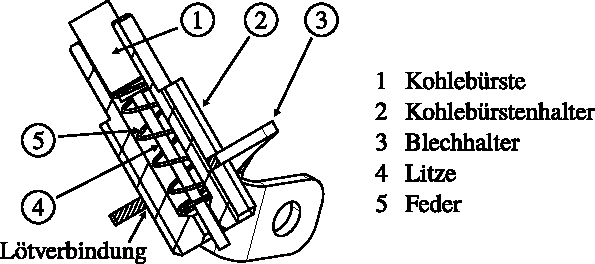
\includegraphics[]{./images/kohlebuerstenhalter_asm.pdf}
    \caption{Die Baugruppe des Kohlebürstenhalters}
    \label{fig:die_baugruppe_des_kohlebuerstenhalters}
\end{figure}
%

Um der elektrische Kontakt zwischen der Kugel und der Messprobe während der Versuche geringe Störungen zu halten, sind zwei Kohlebürsten für die Kugel zu versehen.
Abbildung \ref{fig:der_zusammenbau_des_gesamten_kugelsupports} zeigt den Zusammenbau des Kugelsupports mit der Kugel.
% ----------------------------------------
% Fig: Zusammenbau des gesamten Kugelsupports
% ----------------------------------------
\begin{figure}[htb]
    \centering
    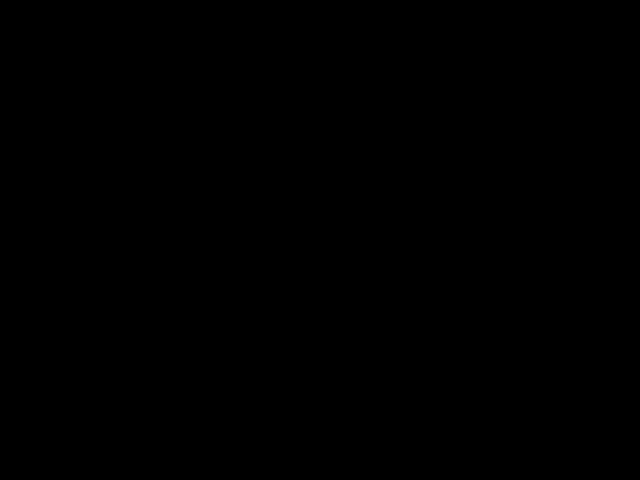
\includegraphics[width=4cm]{./images/blank_img.jpg}
    \caption{Der Zusammenbau des gesamten Kugelsupports}
    \label{fig:der_zusammenbau_des_gesamten_kugelsupports}
\end{figure}
%

% ----------------------------------------
% Sec: Die Glasscheibebaugruppe
% ----------------------------------------
\section{Die Glasscheibebaugruppe}
\label{sec:die_glasscheibebaugruppe}

Blah blah blah
